\title{Lecture 12\\Representation of Subject Domains in a Knowledge Base}

\begin{frame}
	\titlepage
\end{frame}

\begin{frame}{\\Lecture outline}
	\topline
	\justifying
	The concept of knowledge and its classification. Subject domains, their structural specification, and the roles of concepts within them. Child and related subject domains, and types of child subject domains. Types of subject domain hierarchies and intersections between subject domains.
\end{frame}

\begin{frame}{\\Knowledge}
	\topline
	\justifying
	\begin{SCn}
		\scnheader{knowledge}
		\scnidtf{an information construct that is syntactically valid in its language and semantically coherent}
		\scnsubset{information construct}
		\scnrelfrom{covering}{
			type of knowledge\\
			\scnidtf{the set of \underline{all possible} types of knowledge}
			\scntext{note}{The family of \textit{types of knowledge} is a \textit{covering} of the set of all possible items of \textit{knowledge}. This means that every item of \textit{knowledge} belongs to at least one of the identified \textit{types of knowledge}.}
		}
	\end{SCn}
\end{frame}

\begin{frame}{\\Types of knowledge}
	\topline
	\justifying
	\vspace{5mm}
	\footnotesize{
		\begin{SCn}
			\scnheader{type of knowledge}
			\scnhaselement{specification}
			\begin{scnindent}
				\scnidtf{description of a given entity}
				\scnsuperset{specification of a material entity}
				\scnsuperset{specification of an inverse entity that is not a set}
				\scnsuperset{specification of a set}
				\scnsuperset{semantic neighborhood}
				\scnsuperset{unambiguous specification}
				\scnsuperset{comparative analysis}
				\scnsuperset{advantages}
				\scnsuperset{disadvantages}
				\scnsuperset{structure of the entity being specified}
				\scnsuperset{underlying principles}
				\scnsuperset{justification of the proposed solution}
			\end{scnindent}
			\scnhaselement{comparison}
			\scnhaselement{proposition}
			\scnhaselement{formal theory}
			\scnhaselement{subject domain}
		\end{SCn}
	}
\end{frame}

\begin{frame}{\\Types of knowledge}
	\topline
	\justifying
	\begin{SCn}
		\scnheader{type of knowledge}
		\scnhaselement{subject domain and ontology}
		\scnhaselement{metaknowledge}
		\scnhaselement{problem}
		\scnhaselement{plan}
		\scnhaselement{protocol}
		\scnhaselement{results section of a protocol}
		\scnhaselement{method}
		\scnhaselement{technology}
	\end{SCn}
\end{frame}

\begin{frame}{\\Classification of knowledge}
	\topline
	\justifying
	\vspace{5mm}
	\footnotesize{
		\begin{SCn}
			\scnheader{knowledge}
			\begin{scnrelfromset}{partition}
				\scnitem{declarative knowledge}
					\begin{scnindent}
						\scnidtf{\textit{knowledge} with \underline{only} \textit{denotational semantics}, represented by a semantic \textit{specification} of the system of \textit{concepts} it uses}
					\end{scnindent}
				\scnitem{procedural knowledge}
					\begin{scnindent}
						\scnidtf{\textit{knowledge} with both \textit{denotational semantics} and \textit{operational semantics}; the latter is represented by a family of \textit{specifications of agents} that interpret the \textit{procedural knowledge} to solve a \textit{problem} that has been initiated}
						\scnidtf{functionally interpretable knowledge that enables the solution of either a specific problem or a set of problems as they arise}
						\scnsuperset{problem}
						\scnsuperset{plan}
						\scnsuperset{method}
						\scnsuperset{skill}
					\end{scnindent}
			\end{scnrelfromset}
		\end{SCn}
	}
\end{frame}

\begin{frame}{\\Classification of knowledge}
	\topline
	\justifying
	\footnotesize{
		\begin{SCn}
			\scnheader{problem}
			\scnidtf{formulation of a specific problem}
			\scnsuperset{declarative formulation of a problem}
			\scnsuperset{procedural formulation of a problem}
			\scnheader{plan}
			\scnidtf{plan for solving a specific problem}
			\scnidtf{context of a specific problem that provides all the information needed to solve its subproblems}
			\scnidtf{description of the system of subproblems of a given problem}
			\scnheader{method}
			\scnidtf{general description of a plan for solving any problem in a given class of problems}
			\scnheader{skill}
			\scnidtf{method specified down to the level of elementary subproblems}
		\end{SCn}
	}
\end{frame}

\begin{frame}{\\Subject domain}
	\topline
	\justifying
	\begin{SCn}
		\scnheader{subject domain}
		\scnidtf{sc-model of a subject domain}
		\scnidtf{sc-text of a subject domain}
		\scnidtf{sc-graph of a subject domain}
		\scnidtf{representation of a subject domain in \textit{SC-code}}
		\scnsubset{knowledge}
		\scnsubset{infinite set}
		\scntext{explanation}{A \textbf{\textit{subject domain}} is the result of integrating (taking the union of) partial semantic neighborhoods that describe all the entities under study in a given class and share a common subject of study. In other words, the tuples in the neighborhoods being integrated must belong to the same specified set of relations.}
	\end{SCn}
\end{frame}

\begin{frame}{\\Subject domain}
	\topline
	\justifying
	\\
	\footnotesize{
		A \textbf{\textit{subject domain}} is a \textit{structure} that includes:
		\begin{textitemize}
			\item{\textnormal{the main objects under study (or being described), both primary and secondary;}}
			\item{\textnormal{various classes of objects of study;}}
			\item{\textnormal{various tuples whose components are primary or secondary objects of study and may also include other such tuples. Like the objects of study, the tuples can occur at different structural levels;}}
			\item{\textnormal{various classes of those tuples, i.e., relations;}}
			\item{\textnormal{various classes of objects that serve as components of those tuples without themselves being objects of study or tuples of the kind described above.}}
		\end{textitemize}
		All classes designated as concepts under study must be represented in full within the subject domain, together with their elements, the elements of those elements, and so on down to the terminal elements.
	}
\end{frame}

\begin{frame}{\\Role of a subject domain element}
	\topline
	\justifying
	\begin{SCn}
		\scnheader{role of a subject domain element}
		\scnidtf{role relation linking subject domains to their key signs}
		\scnidtf{role of a key element (a sign denoting a key entity) of a subject domain}
		\scnidtf{role of a key sign of a subject domain}
		\scnhaselement{class of objects of study\scnrolesign}
		\scnhaselement{maximal class of objects of study\scnrolesign}
		\scnhaselement{key object of study\scnrolesign}
		\scnhaselement{concept used in a subject domain\scnrolesign}
		\scnhaselement{primary element under study in a subject domain\scnrolesign}
		\scnhaselement{secondary element under study in a subject domain\scnrolesign}
		\scnhaselement{element outside the scope of study in a subject domain\scnrolesign}
	\end{SCn}
\end{frame}

\begin{frame}{\\Class of objects of study}
	\topline
	\justifying
	\footnotesize{
		\begin{SCn}
			\scnheader{class of objects of study\scnrolesign}
			\scnidtf{being a class of \underline{primary} objects of study in the given subject domain\scnrolesign}
			\scntext{note}{Whether an object of study is \underline{primary} is \underline{relative} to the subject domain and is independent of the object's type and complexity.

			The most general \textit{classes of objects of study}, which correspond to \underline{high-level} \textit{subject domains and ontologies}, require particular attention. The set of all entities around us should be decomposed into a carefully designed hierarchy of \textit{classes of objects of study}. This hierarchy corresponds to a hierarchy of \textit{subject domains and ontologies}, which determines how the objects under study \underline{inherit properties}.}
			\scnrelfrom{second domain}{class}
		\end{SCn}
	}
\end{frame}

\begin{frame}{\\Class of objects of study}
	\topline
	\justifying
	\begin{SCn}
		\scnheader{maximal class of objects of study\scnrolesign}
		\scnidtf{class of objects of study that is not a proper subset of any other class of objects of study \underline{in the given} subject domain\scnrolesign}
		\scntext{note}{A subject domain may have \underline{several} maximal classes of objects of study.}
		\scnheader{key object of study\scnrolesign}
		\scnidtf{special object of study\scnrolesign}
		\scnidtf{being a sign of a special object under study within the given subject domain\scnrolesign}
		\scnidtf{object of study with special properties\scnrolesign}
	\end{SCn}
\end{frame}

\begin{frame}{\\Key element of a subject domain}
	\topline
	\justifying
	\begin{SCn}
		\scnheader{key element of a subject domain\scnrolesign}
		\scnidtf{sign of a key entity that is part of the subject domain\scnrolesign}
		\begin{scnrelfromset}{partition}
			\scnitem{concept used in a subject domain\scnrolesign}
			\scnitem{key object of study\scnrolesign}
		\end{scnrelfromset}
	\end{SCn}
\end{frame}

\begin{frame}{\\Concept used in a subject domain}
	\topline
	\justifying
	\begin{SCn}
		\scnheader{concept used in a subject domain\scnrolesign}
		\scnidtf{concept that serves as a \underline{key} concept in the given subject domain rather than as an object of study\scnrolesign}
		\scnsubset{concept used\scnrolesign}
		\scnrelfrom{partition}{semantic type of the concept used}
		\begin{scnindent}
			\begin{scneqtoset}
				\scnitem{class of objects of study\scnrolesign}
				\scnitem{relation used in a subject domain\scnrolesign}
				\scnitem{class of structures used in a subject domain\scnrolesign}
			\end{scneqtoset}
		\end{scnindent}
	\end{SCn}
\end{frame}

\begin{frame}{\\Concept used in a subject domain}
	\topline
	\justifying
	\begin{SCn}
		\scnheader{concept used in a subject domain\scnrolesign}
		\scnrelfrom{partition}{completeness of inclusion of the concept's elements in the subject domain}
		\begin{scnindent}
			\begin{scneqtoset}
				\scnitem{concept used whose elements all belong to the given subject domain\scnrolesign}
				\scnitem{concept used whose elements do not all belong to the given subject domain\scnrolesign}
			\end{scneqtoset}
		\end{scnindent}
		\scnrelfrom{partition}{whether the concept is first introduced here}
		\begin{scnindent}
			\begin{scneqtoset}
				\scnitem{concept introduced in the given subject domain\scnrolesign}
				\scnitem{concept used but not introduced in the given subject domain\scnrolesign}
			\end{scneqtoset}
		\end{scnindent}
	\end{SCn}
\end{frame}

\begin{frame}{\\Concept used in a subject domain}
	\topline
	\justifying
	\vspace{5mm}
	\begin{SCn}
		\scnheader{concept used in a subject domain\scnrolesign}
		\scnrelfrom{partition}{whether the concept is defined or declared undefined with a detailed explanation and examples}
		\begin{scnindent}
			\begin{scneqtoset}
				\scnitem{concept defined or declared undefined in the given subject domain\scnrolesign}
				\scnitem{concept with neither a definition nor a declaration that it is undefined in the given subject domain\scnrolesign}
			\end{scneqtoset}
		\end{scnindent}
		\scnrelfrom{partition}{whether the concept is studied}
		\begin{scnindent}
			\begin{scneqtoset}
				\scnitem{concept studied in the given subject domain\scnrolesign}
				\scnitem{concept used but not studied in the given subject domain\scnrolesign}
			\end{scneqtoset}
		\end{scnindent}
	\end{SCn}
\end{frame}

\begin{frame}{\\Primary and secondary elements under study}
	\topline
	\justifying
	\begin{SCn}
		\scnheader{primary element under study in a subject domain\scnrolesign}
		\scnidtf{sign of a primary object of study within the given subject domain\scnrolesign}
		\scnheader{secondary element under study in a subject domain\scnrolesign}
		\scnidtf{sign of a secondary object of study within the subject domain\scnrolesign}
		\scnsuperset{tuple of subject domain elements\scnrolesign}
		\scnsuperset{class of subject domain elements\scnrolesign}
		\scnsuperset{structure of subject domain elements\scnrolesign}
	\end{SCn}
\end{frame}

\begin{frame}{\\Elements outside the scope of study}
	\topline
	\justifying
	\footnotesize{
		\begin{SCn}
			\scnheader{element outside the scope of study in a subject domain\scnrolesign}
			\scnidtf{auxiliary element of the subject domain that is studied in another (related) subject domain\scnrolesign}
			\scntext{note}{Elements outside the scope of study help describe and investigate various kinds of connections between elements studied in the given \textit{subject domain} and elements studied in other \textit{subject domains}.

			A \textit{tuple} containing both kinds of elements is itself \underline{under study} in the given \textit{subject domain}.

			In a \textit{subject domain} of geometry, examples of elements outside the scope of study include \textit{numbers} that serve as \textit{values of quantities} such as \textit{distance}\scnsupergroupsign, \textit{length}\scnsupergroupsign, \textit{area}\scnsupergroupsign, and \textit{volume}\scnsupergroupsign. Other examples include numerical \textit{relations} (\textit{addition}*, \textit{multiplication}*, \textit{exponentiation}*) and set-theoretic \textit{relations} (\textit{inclusion}*, \textit{union}*, \textit{intersection}*, \textit{membership}*).}
		\end{SCn}
	}
\end{frame}

\begin{frame}{\\Concept}
	\topline
	\justifying
	\small{
		\begin{SCn}
			\scnheader{concept}
			\scnidtf{notion}
			\scnidtf{class of entities that serves as a key concept under study in at least one subject domain}
			\scntext{note}{The family of all concepts that have been introduced forms a kind of semantic coordinate system for specifying entities of all kinds in semantic space.}
			\scnidtf{class of entities designated as a \textit{concept} (introduced, studied, or auxiliary) in at least one \textit{subject domain}}
			\scntext{note}{Every \textit{concept} has at least one \textit{subject domain} in which it is a \textit{concept under study} and its main characteristics are examined. A \textit{subject domain} that needs to examine additional connections between this \textit{concept} and other \textit{concepts} designates it as an \textit{auxiliary concept}\scnrolesign.}
		\end{SCn}
	}
\end{frame}

\begin{frame}{\\Concept}
	\topline
	\justifying
	\begin{SCn}
		\scnheader{concept}
		\scnidtf{second domain of the \textit{concept used}* relation}
		\scnrelto{second domain}{concept used*}
		\scnidtf{class of entities (a class of tuples such as a relation, a class of classes such as a parameter, or a class of structures) that is a \textit{concept used} in at least one \textit{subject domain}\scnrolesign}
	\end{SCn}
\end{frame}

\begin{frame}{\\Relations on the set of subject domains}
	\topline
	\justifying
	\begin{SCn}
		\scnheader{relation defined on the set of subject domains}
		\scnhaselement{\scnkeyword{child subject domain*}}
		\scnhaselement{\scnkeyword{integration of subject domains*}}
		\scnhaselement{\scnkeyword{isomorphism of subject domains*}}
		\scnhaselement{\scnkeyword{homomorphism of subject domains*}}
	\end{SCn}
\end{frame}

\begin{frame}{\\Child subject domain}
	\topline
	\justifying
	\vspace{5mm}
	\begin{SCn}
		\scnheader{child subject domain*}
		\scnidtf{specialized subject domain*}
		\scnidtf{being a specialized subject domain*}
		\scnidtf{direct descendant of a subject domain*}
		\scnidtf{narrowing a subject domain by class of objects of study*}
		\scnidtf{subject domain that describes in greater detail one of the classes of objects of study of another, more general subject domain*}
		\scnidtf{subject domain for which the union of its classes of objects of study is a subset of the corresponding union for the given subject domain*}
		\scniselement{binary relation}
		\scniselement{directed relation}
		\scniselement{non-role relation}
		\scnsuperset{child subject domain by class of primary elements*}
		\scnsuperset{child subject domain by relations under study*}
	\end{SCn}
\end{frame}

\begin{frame}{\\Child subject domain}
	\topline
	\justifying
	\begin{SCn}
		\scnheader{child subject domain*}
		\scntext{explanation}{\textit{Child subject domain*} is a binary directed relation that defines a hierarchy of subject domains by moving from a less detailed to a more detailed study of the corresponding concepts.}
		\scntext{note}{All \textit{child subject domains*} of a \textit{subject domain} \underline{inherit} all the properties of its \textit{objects of study}.}
	\end{SCn}
\end{frame}

\begin{frame}{}
	\topline
	\justifying
	\small{
		\begin{SCn}
			\scnheader{extension of the family of relations under study*}
			\scntext{explanation}{Moving from one subject domain to another with the same maximal class of objects of study, but with an expanded family of relations and possibly an expanded family of explicitly identified classes of objects of study (subclasses of the maximal class).}
			\scnheader{transition to studying the internal structure of objects of study*}
			\scntext{explanation}{Moving from the study of external connections between objects of study to the study of their internal structure by decomposing the objects into parts and including those parts among the objects of study.}
		\end{SCn}
	}
\end{frame}

\begin{frame}{}
	\topline
	\justifying
	\begin{SCn}
		\scnheader{transition to studying structures made up of objects of study*}
		\scntext{explanation}{Moving from describing a given class of objects of study to describing the class of all sets whose elements are those objects. An example is the transition from the subject domain of geometric points to the subject domain of geometric figures.}
	\end{SCn}
\end{frame}

\begin{frame}{\\Example of a subject domain hierarchy}
	\topline
	\justifying
	\vspace{10mm}

	\begin{center}
		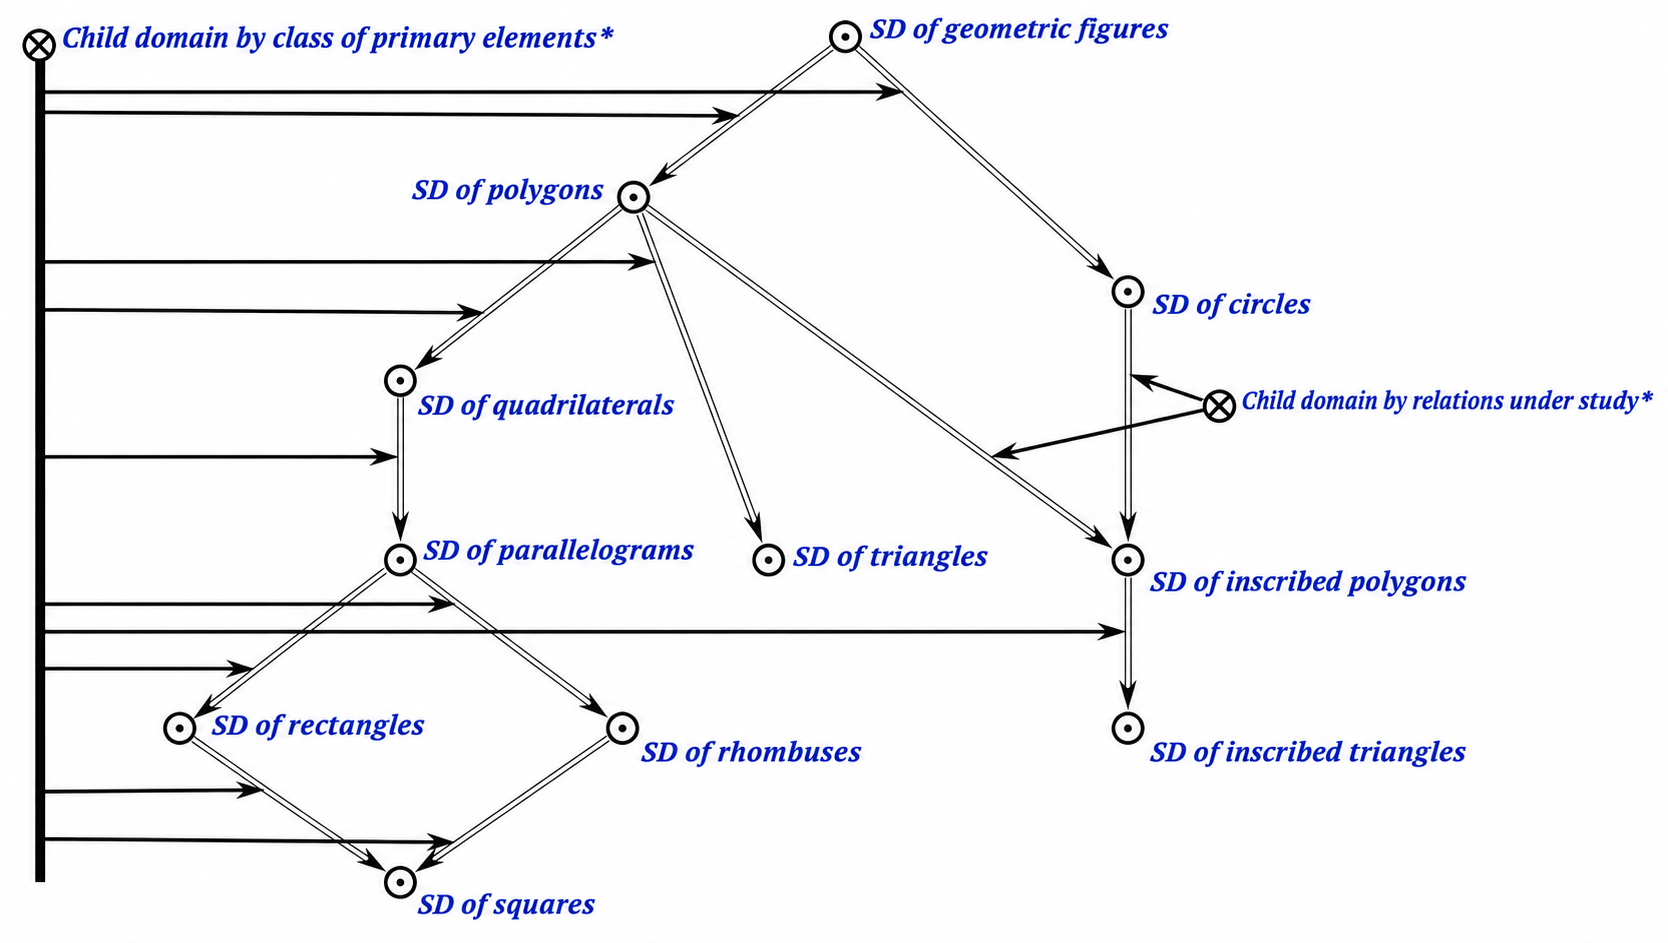
\includegraphics[width=\linewidth,height=0.67\textheight,keepaspectratio]{figures/sd_sd/sd_hierarchy_en.png}
	\end{center}
\end{frame}
